%
% dido.tex
%
% (c) 2023 Prof Dr Andreas Müller
%
\begin{figure}
\centering
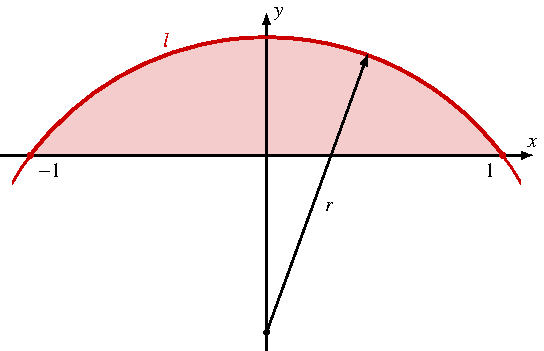
\includegraphics{chapters/050-nebenbedingungen/images/dido.pdf}
\caption{Problem der Dido in der Ebene.
Gesucht wird die Kurve gegebener Länge $l$ zwischen den Punkten $(\pm 1,0)$,
die mit der $x$-Achse den grössten Flächeninhalt einschliesst.
\label{buch:nebenbedingungen:lagrangemult:fig:dido}}
\end{figure}
